\documentclass[aspectratio=169,11pt]{beamer}

% TEMA Y COLORES
\usetheme{Madrid}
\usecolortheme{whale}

\definecolor{primaryblue}{RGB}{0,102,153}
\definecolor{accentgreen}{RGB}{0,128,0}
\definecolor{accentorange}{RGB}{204,102,0}
\definecolor{darkgray}{RGB}{64,64,64}

\setbeamercolor{palette primary}{bg=primaryblue,fg=white}
\setbeamercolor{palette secondary}{bg=primaryblue!80,fg=white}
\setbeamercolor{palette tertiary}{bg=primaryblue!60,fg=white}
\setbeamercolor{structure}{fg=primaryblue}
\setbeamercolor{block title}{bg=primaryblue,fg=white}
\setbeamercolor{block body}{bg=primaryblue!10}
\setbeamercolor{block title example}{bg=accentgreen,fg=white}
\setbeamercolor{block body example}{bg=accentgreen!10}
\setbeamercolor{block title alerted}{bg=accentorange,fg=white}
\setbeamercolor{block body alerted}{bg=accentorange!10}

% PAQUETES
\usepackage[utf8]{inputenc}
\usepackage[T1]{fontenc}
\usepackage{amsmath,amssymb}
\usepackage{booktabs}
\usepackage{tikz}
\usepackage{pgfplots}
\usepackage{listings}
\usepackage{multicol}

\pgfplotsset{compat=1.17}
\lstset{literate={ñ}{{\~n}}1 {á}{{\'a}}1 {é}{{\'e}}1 {í}{{\'i}}1 {ó}{{\'o}}1 {ú}{{\'u}}1}

% CÓDIGO PYTHON
\lstdefinestyle{pythonstyle}{
    language=Python,
    basicstyle=\ttfamily\footnotesize,
    keywordstyle=\color{blue}\bfseries,
    stringstyle=\color{red},
    commentstyle=\color{accentgreen}\itshape,
    frame=single,
    breaklines=true,
    showstringspaces=false,
    backgroundcolor=\color{gray!10}
}

% NAVEGACIÓN Y PIE DE PÁGINA
\setbeamertemplate{navigation symbols}{}
\setbeamertemplate{footline}{
    \leavevmode%
    \hbox{%
        \begin{beamercolorbox}[wd=.333333\paperwidth,ht=2.25ex,dp=1ex,center]{author in head/foot}%
            \usebeamerfont{author in head/foot}Matemáticas Financieras
        \end{beamercolorbox}%
        \begin{beamercolorbox}[wd=.333333\paperwidth,ht=2.25ex,dp=1ex,center]{title in head/foot}%
            \usebeamerfont{title in head/foot}Sesión 2
        \end{beamercolorbox}%
        \begin{beamercolorbox}[wd=.333333\paperwidth,ht=2.25ex,dp=1ex,right]{date in head/foot}%
            \usebeamerfont{date in head/foot}\insertframenumber{} / \inserttotalframenumber\hspace*{2ex}
        \end{beamercolorbox}}%
    \vskip0pt%
}

\title[Sesión 2]{Valor Presente y Descuento}
\subtitle{El proceso inverso de la capitalización}
\author{Matemáticas Financieras}
\institute{Valor del Dinero en el Tiempo}
\date{Semana 1 | Clase 2 | Duración: 1h 50min}

\begin{document}

% ===========================================
% SECCIÓN 1: PORTADA Y CONTENIDO
% ===========================================

\begin{frame}
    \titlepage
\end{frame}

\begin{frame}{Contenido de la Sesión}
    \tableofcontents
\end{frame}

% ===========================================
% SECCIÓN 2: INTRODUCCIÓN
% ===========================================
\section{Introducción}

\begin{frame}{Conexión con la Sesión Anterior}
    \begin{block}{Sesión 1: Capitalización}
        Aprendimos a mover el dinero \textbf{hacia adelante} en el tiempo:
        \[
        F = P(1 + r)^n
        \]
        Dado un valor presente $P$, calculamos su valor futuro $F$.
    \end{block}

    \pause
    \vspace{0.5cm}

    \begin{exampleblock}{Sesión 2: Descuento}
        Hoy aprenderemos el proceso \textbf{inverso}: mover el dinero \textbf{hacia atrás} en el tiempo.

        \textbf{Pregunta clave:} ¿Cuánto vale HOY un pago que recibiré en el FUTURO?
    \end{exampleblock}
\end{frame}

\begin{frame}{Objetivos de Aprendizaje}
    Al finalizar esta sesión, serás capaz de:
    \begin{enumerate}
        \item Comprender el concepto de valor presente y su derivación
        \item Aplicar el factor de descuento para traer valores al presente
        \item Distinguir entre tasa de descuento y tasa de interés
        \item Construir e interpretar diagramas de flujo de caja
        \item Diferenciar entre descuento simple y descuento compuesto
        \item Calcular el valor presente de flujos futuros con HP 12C y Python
    \end{enumerate}
\end{frame}

\begin{frame}{Motivación: ¿Cuánto Pagarías Hoy?}
    \begin{block}{Pregunta}
        Te prometen pagar \$10,000 dentro de 5 años con certeza. Si puedes invertir al 8\% anual, ¿cuál es el \textbf{máximo} que pagarías hoy por ese derecho?
    \end{block}

    \pause
    \vspace{0.5cm}

    \textbf{Razonamiento:}
    \begin{itemize}
        \item<2-> Si pagas $X$ hoy, en 5 años tendrás: $X(1.08)^5$
        \item<3-> Para que valga la pena: $X(1.08)^5 \geq \$10,000$
        \item<4-> El punto de indiferencia: $X = \$10,000 / (1.08)^5$
        \item<5-> $X = \$10,000 / 1.4693 = \$6,805.83$
    \end{itemize}

    \pause[6]
    \begin{exampleblock}{Conclusión}
        \$6,805.83 hoy es \textbf{equivalente} a \$10,000 en 5 años (al 8\%).
    \end{exampleblock}
\end{frame}

\begin{frame}{Definiciones Clave}
    \begin{block}{Valor Presente ($P$ o $PV$)}
        Valor actual de un flujo de dinero futuro, descontado a una tasa apropiada.
    \end{block}

    \pause

    \begin{block}{Factor de Descuento}
        El término $\dfrac{1}{(1+r)^n}$ que ``reduce'' el valor futuro al presente.
    \end{block}

    \pause

    \begin{block}{Tasa de Descuento ($r$)}
        Tasa utilizada para calcular el valor presente. Refleja el costo de oportunidad del dinero.
    \end{block}

    \pause

    \begin{alertblock}{Nota Importante}
        Descontar es el proceso de encontrar el valor presente de un flujo futuro.
    \end{alertblock}
\end{frame}

% ===========================================
% SECCIÓN 3: DERIVACIONES MATEMÁTICAS
% ===========================================
\section{Derivación del Valor Presente}

\begin{frame}{De Capitalización a Descuento}
    \textbf{Partimos de la fórmula de valor futuro:}
    \[
    F = P(1 + r)^n
    \]

    \pause
    \vspace{0.3cm}

    \textbf{Despejamos el valor presente $P$:}
    \begin{align*}
        F &= P(1 + r)^n \\[0.3cm]
        \pause
        \frac{F}{(1 + r)^n} &= P \\[0.3cm]
        \pause
        P &= F \cdot \frac{1}{(1 + r)^n}
    \end{align*}

    \pause
    \begin{block}{Fórmula del Valor Presente}
        \[
        \boxed{P = \frac{F}{(1 + r)^n} = F \cdot (1 + r)^{-n}}
        \]
    \end{block}
\end{frame}

\begin{frame}{El Factor de Descuento}
    Definimos el \textbf{factor de descuento} como:
    \[
    \boxed{DF = \frac{1}{(1 + r)^n} = (1 + r)^{-n}}
    \]

    \pause
    \vspace{0.3cm}

    \textbf{Propiedades del factor de descuento:}
    \begin{itemize}
        \item<2-> Siempre está entre 0 y 1 (para $r > 0$)
        \item<3-> Cuando $n = 0$: $DF = 1$ (no hay descuento)
        \item<4-> A mayor $n$: menor $DF$ (más lejos = menos valor hoy)
        \item<5-> A mayor $r$: menor $DF$ (mayor costo de oportunidad)
    \end{itemize}

    \pause[6]
    \vspace{0.3cm}

    \textbf{Relación con el factor de capitalización:}
    \[
    \text{Factor de descuento} = \frac{1}{\text{Factor de capitalización}}
    \]
\end{frame}

\begin{frame}{Factor de Descuento vs. Factor de Capitalización}
    \begin{center}
    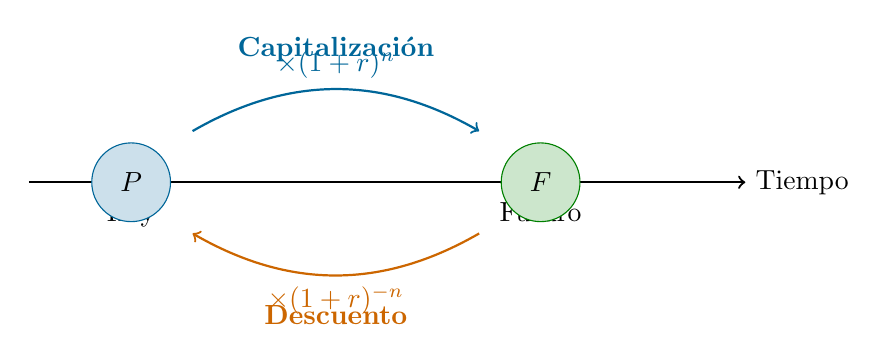
\begin{tikzpicture}[scale=1.3]
        % Línea de tiempo
        \draw[thick, ->] (0,0) -- (7,0) node[right] {Tiempo};

        % Marcas
        \draw (1,0.1) -- (1,-0.1) node[below] {Hoy};
        \draw (5,0.1) -- (5,-0.1) node[below] {Futuro};

        % Valor presente
        \node[circle, draw=primaryblue, fill=primaryblue!20, minimum size=1cm] at (1,0) {$P$};

        % Valor futuro
        \node[circle, draw=accentgreen, fill=accentgreen!20, minimum size=1cm] at (5,0) {$F$};

        % Flechas
        \draw[->, thick, primaryblue] (1.6,0.5) to[bend left=30] node[above] {$\times (1+r)^n$} (4.4,0.5);
        \draw[->, thick, accentorange] (4.4,-0.5) to[bend left=30] node[below] {$\times (1+r)^{-n}$} (1.6,-0.5);

        % Etiquetas
        \node[primaryblue] at (3,1.3) {\textbf{Capitalización}};
        \node[accentorange] at (3,-1.3) {\textbf{Descuento}};
    \end{tikzpicture}
    \end{center}

    \pause
    \vspace{0.3cm}

    \begin{columns}
        \begin{column}{0.5\textwidth}
            \textbf{Capitalización:}
            \[F = P \cdot (1+r)^n\]
            Mover hacia el futuro
        \end{column}
        \begin{column}{0.5\textwidth}
            \textbf{Descuento:}
            \[P = F \cdot (1+r)^{-n}\]
            Mover hacia el presente
        \end{column}
    \end{columns}
\end{frame}

\begin{frame}{Tasa de Descuento vs. Tasa de Interés}
    \begin{block}{¿Son lo mismo?}
        Matemáticamente, usamos el mismo valor $r$, pero conceptualmente tienen interpretaciones distintas:
    \end{block}

    \pause
    \vspace{0.3cm}

    \begin{columns}
        \begin{column}{0.48\textwidth}
            \textbf{Tasa de Interés}
            \begin{itemize}
                \item Perspectiva del prestamista
                \item Lo que \textbf{ganas} por prestar
                \item Mide el crecimiento del dinero
            \end{itemize}
        \end{column}

        \begin{column}{0.48\textwidth}
            \textbf{Tasa de Descuento}
            \begin{itemize}
                \item Perspectiva del inversionista
                \item El \textbf{costo de oportunidad}
                \item Mide la pérdida de valor en el tiempo
            \end{itemize}
        \end{column}
    \end{columns}

    \pause
    \vspace{0.5cm}

    \begin{alertblock}{En la práctica}
        La tasa de descuento refleja el \textbf{rendimiento mínimo requerido} que exige un inversionista para aceptar un flujo futuro.
    \end{alertblock}
\end{frame}

\begin{frame}{Tabla de Factores de Descuento}
    \textbf{Factores de descuento $(1+r)^{-n}$ para valores comunes:}

    \vspace{0.3cm}

    \begin{center}
    \begin{tabular}{@{}c|ccccc@{}}
        \toprule
        $r$ \textbackslash{} $n$ & 1 & 5 & 10 & 15 & 20 \\
        \midrule
        5\% & 0.9524 & 0.7835 & 0.6139 & 0.4810 & 0.3769 \\
        8\% & 0.9259 & 0.6806 & 0.4632 & 0.3152 & 0.2145 \\
        10\% & 0.9091 & 0.6209 & 0.3855 & 0.2394 & 0.1486 \\
        12\% & 0.8929 & 0.5674 & 0.3220 & 0.1827 & 0.1037 \\
        15\% & 0.8696 & 0.4972 & 0.2472 & 0.1229 & 0.0611 \\
        \bottomrule
    \end{tabular}
    \end{center}

    \pause
    \vspace{0.3cm}

    \begin{exampleblock}{Ejemplo de uso}
        VP de \$10,000 en 10 años al 10\%: $P = \$10,000 \times 0.3855 = \$3,855$
    \end{exampleblock}
\end{frame}

% ===========================================
% SECCIÓN 4: DIAGRAMAS DE FLUJO
% ===========================================
\section{Diagramas de Flujo de Caja}

\begin{frame}{¿Qué es un Diagrama de Flujo de Caja?}
    \begin{block}{Definición}
        Representación gráfica de los flujos de dinero a lo largo del tiempo, mostrando el momento y la dirección de cada flujo.
    \end{block}

    \pause
    \vspace{0.3cm}

    \textbf{Elementos del diagrama:}
    \begin{itemize}
        \item \textbf{Línea horizontal:} Eje del tiempo (períodos)
        \item \textbf{Flechas hacia arriba:} Entradas de dinero (positivas)
        \item \textbf{Flechas hacia abajo:} Salidas de dinero (negativas)
        \item \textbf{Longitud de flechas:} Proporcional al monto
    \end{itemize}

    \pause
    \vspace{0.3cm}

    \begin{alertblock}{Importancia}
        Los diagramas ayudan a visualizar problemas complejos y evitar errores de signo.
    \end{alertblock}
\end{frame}

\begin{frame}{Ejemplo: Inversión Simple}
    \textbf{Situación:} Inviertes \$5,000 hoy y recibes \$7,000 en 3 años.

    \begin{center}
        \begin{tikzpicture}[scale=1.1]
            % Línea de tiempo
            \draw[thick, ->] (-0.5,0) -- (7,0) node[right] {Años};

            % Marcas de tiempo
            \foreach \x/\label in {0/0, 2/1, 4/2, 6/3} {
                \draw (\x,0.1) -- (\x,-0.1) node[below] {\label};
            }

            % Inversión inicial (salida)
            \draw[thick, ->, primaryblue] (0,0) -- (0,-1.5);
            \node[primaryblue, below] at (0,-1.6) {\$5,000};

            % Retorno (entrada)
            \draw[thick, ->, accentgreen] (6,0) -- (6,1.8);
            \node[accentgreen, above] at (6,1.9) {\$7,000};

            % Etiquetas
            \node[primaryblue] at (0,-2.3) {\footnotesize Inversión};
            \node[accentgreen] at (6,2.6) {\footnotesize Retorno};
        \end{tikzpicture}
    \end{center}

    \pause
    \vspace{0.3cm}

    \textbf{Pregunta:} ¿Es buena inversión si el costo de oportunidad es 12\%?
\end{frame}

\begin{frame}{Análisis del Ejemplo}
    \textbf{Método 1: Llevar todo al futuro}
    \begin{align*}
        VF_{\text{inversión}} &= \$5,000 \times (1.12)^3 = \$5,000 \times 1.4049 = \$7,025
    \end{align*}

    Como \$7,025 > \$7,000, \textbf{no} es buena inversión (ganas menos de lo que podrías).

    \pause
    \vspace{0.5cm}

    \textbf{Método 2: Llevar todo al presente}
    \begin{align*}
        VP_{\text{retorno}} &= \$7,000 \times (1.12)^{-3} = \$7,000 \times 0.7118 = \$4,983
    \end{align*}

    Como \$4,983 < \$5,000, \textbf{no} es buena inversión (el VP del retorno es menor que la inversión).

    \pause
    \vspace{0.3cm}

    \begin{exampleblock}{Ambos métodos dan la misma respuesta}
        Siempre debemos comparar valores en el \textbf{mismo punto del tiempo}.
    \end{exampleblock}
\end{frame}

\begin{frame}{Diagrama con Múltiples Flujos}
    \textbf{Situación:} Recibes \$2,000 al final del año 1, \$3,000 al final del año 2, y \$4,000 al final del año 3.

    \begin{center}
        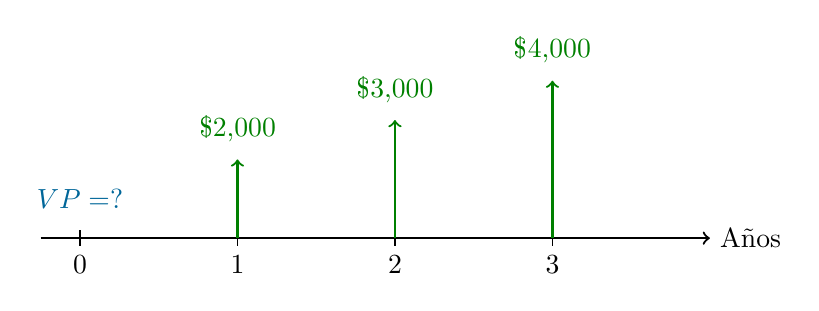
\begin{tikzpicture}[scale=1.0]
            % Línea de tiempo
            \draw[thick, ->] (-0.5,0) -- (8,0) node[right] {Años};

            % Marcas de tiempo
            \foreach \x/\label in {0/0, 2/1, 4/2, 6/3} {
                \draw (\x,0.1) -- (\x,-0.1) node[below] {\label};
            }

            % Flujos
            \draw[thick, ->, accentgreen] (2,0) -- (2,1.0);
            \node[accentgreen, above] at (2,1.1) {\$2,000};

            \draw[thick, ->, accentgreen] (4,0) -- (4,1.5);
            \node[accentgreen, above] at (4,1.6) {\$3,000};

            \draw[thick, ->, accentgreen] (6,0) -- (6,2.0);
            \node[accentgreen, above] at (6,2.1) {\$4,000};

            % VP
            \node[primaryblue] at (0,0.5) {$VP = ?$};
        \end{tikzpicture}
    \end{center}

    \pause
    \vspace{0.3cm}

    \textbf{Valor Presente Total (al 10\%):}
    \begin{align*}
        VP &= \frac{2,000}{(1.10)^1} + \frac{3,000}{(1.10)^2} + \frac{4,000}{(1.10)^3} \\
        VP &= 1,818 + 2,479 + 3,005 = \$7,302
    \end{align*}
\end{frame}

% ===========================================
% SECCIÓN 5: DESCUENTO SIMPLE VS COMPUESTO
% ===========================================
\section{Descuento Simple vs. Compuesto}

\begin{frame}{Descuento Simple (Comercial)}
    \begin{block}{Definición}
        En el \textbf{descuento simple}, el descuento se calcula sobre el valor nominal (futuro) del documento.
    \end{block}

    \pause
    \vspace{0.3cm}

    \textbf{Fórmula del descuento simple:}
    \[
    D = F \cdot d \cdot n
    \]

    donde $d$ es la \textbf{tasa de descuento} y $D$ es el monto del descuento.

    \pause
    \vspace{0.3cm}

    \textbf{Valor Presente:}
    \[
    \boxed{P = F - D = F(1 - d \cdot n)}
    \]

    \pause
    \begin{alertblock}{Uso común}
        Se utiliza en operaciones de corto plazo: descuento de pagarés, letras de cambio, factoraje.
    \end{alertblock}
\end{frame}

\begin{frame}{Ejemplo: Descuento de un Pagaré}
    \begin{block}{Problema}
        Un pagaré con valor nominal de \$50,000 vence en 90 días. El banco lo descuenta a una tasa de descuento simple del 18\% anual. ¿Cuánto recibe el tenedor hoy?
    \end{block}

    \pause
    \vspace{0.3cm}

    \textbf{Solución:}
    \begin{align*}
        n &= \frac{90}{360} = 0.25 \text{ años} \\[0.2cm]
        D &= F \cdot d \cdot n = 50,000 \times 0.18 \times 0.25 = \$2,250 \\[0.2cm]
        P &= F - D = 50,000 - 2,250 = \$47,750
    \end{align*}

    \pause
    \vspace{0.3cm}

    El tenedor recibe \textbf{\$47,750} hoy a cambio de un pagaré de \$50,000 en 90 días.
\end{frame}

\begin{frame}{Descuento Compuesto (Racional)}
    \begin{block}{Definición}
        En el \textbf{descuento compuesto} (también llamado descuento racional o matemático), usamos la fórmula de valor presente con interés compuesto.
    \end{block}

    \pause
    \vspace{0.3cm}

    \textbf{Fórmula:}
    \[
    \boxed{P = \frac{F}{(1 + r)^n}}
    \]

    donde $r$ es la tasa de interés (no la tasa de descuento).

    \pause
    \vspace{0.3cm}

    \begin{exampleblock}{Uso común}
        Es el método estándar en finanzas para valuar flujos futuros, especialmente en plazos largos.
    \end{exampleblock}
\end{frame}

\begin{frame}{Comparación: Simple vs. Compuesto}
    \textbf{Mismo problema:} VP de \$10,000 a 2 años con tasa del 10\%.

    \pause
    \vspace{0.3cm}

    \textbf{Descuento Simple:}
    \begin{align*}
        P &= F(1 - d \cdot n) = 10,000(1 - 0.10 \times 2) \\
        P &= 10,000 \times 0.80 = \$8,000
    \end{align*}

    \pause
    \textbf{Descuento Compuesto:}
    \begin{align*}
        P &= \frac{F}{(1+r)^n} = \frac{10,000}{(1.10)^2} \\
        P &= \frac{10,000}{1.21} = \$8,264.46
    \end{align*}

    \pause
    \vspace{0.3cm}

    \begin{alertblock}{Observación}
        El descuento simple genera un VP menor (descuenta más). Esta diferencia crece con el tiempo.
    \end{alertblock}
\end{frame}

\begin{frame}{Gráfica Comparativa}
    \begin{center}
        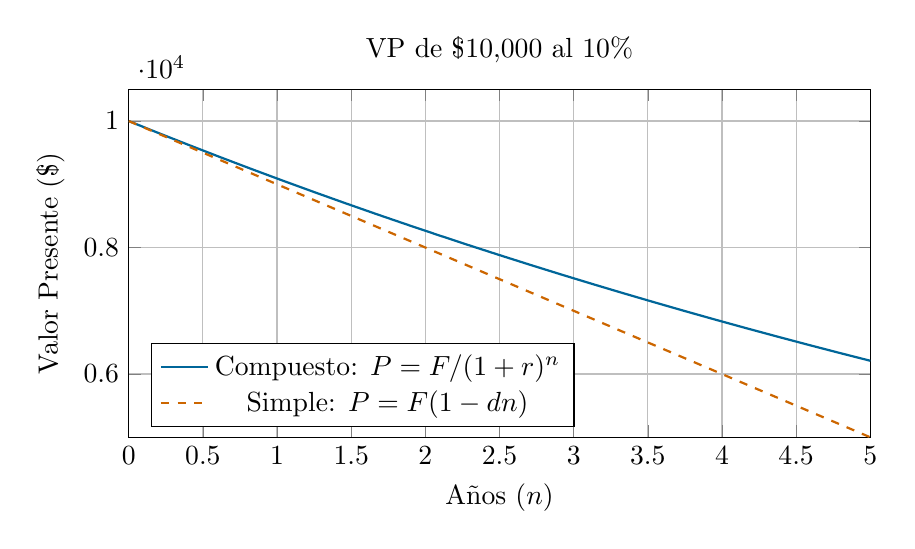
\begin{tikzpicture}
            \begin{axis}[
                xlabel={Años ($n$)},
                ylabel={Valor Presente (\$)},
                xmin=0, xmax=5,
                ymin=5000, ymax=10500,
                grid=major,
                width=11cm,
                height=6cm,
                legend pos=south west,
                title={VP de \$10,000 al 10\%}
            ]
            % Descuento compuesto
            \addplot[color=primaryblue, thick, domain=0:5] {10000/(1.1)^x};
            \addlegendentry{Compuesto: $P = F/(1+r)^n$}
            % Descuento simple
            \addplot[color=accentorange, thick, dashed, domain=0:5] {10000*(1-0.1*x)};
            \addlegendentry{Simple: $P = F(1-dn)$}
            \end{axis}
        \end{tikzpicture}
    \end{center}

    \textbf{Nota:} A partir de $n = 10$ años, el descuento simple daría valores negativos (sin sentido).
\end{frame}

% ===========================================
% SECCIÓN 6: TRUCOS DE ESTIMACIÓN
% ===========================================
\section{Trucos de Estimación Mental}

\begin{frame}{Regla del 72 para Valor Presente}
    \begin{alertblock}{Aplicación Inversa de la Regla del 72}
        Si el dinero se duplica en $72/r\%$ años hacia adelante, también se \textbf{reduce a la mitad} en $72/r\%$ años hacia atrás.
    \end{alertblock}

    \pause
    \vspace{0.5cm}

    \textbf{Ejemplo:} ¿Cuánto vale hoy \$100,000 que recibiré en 9 años al 8\%?

    \pause
    \begin{enumerate}
        \item Tiempo para duplicar al 8\%: $72/8 = 9$ años
        \item Por lo tanto, en 9 años el dinero se duplicaría
        \item Hacia atrás: el valor se reduce a la mitad
        \item $VP \approx \$100,000 / 2 = \$50,000$
    \end{enumerate}

    \pause
    \vspace{0.3cm}

    \textbf{Verificación:} $P = 100,000/(1.08)^9 = 100,000/2.00 = \$50,025$ \checkmark
\end{frame}

\begin{frame}{Estimación por Mitades}
    \textbf{Usando factores de descuento aproximados:}

    \begin{center}
    \begin{tabular}{@{}ccl@{}}
        \toprule
        \textbf{Tasa} & \textbf{Años para $\div 2$} & \textbf{Ejemplo} \\
        \midrule
        6\% & 12 años & \$80,000 en 12 años $\approx$ \$40,000 hoy \\
        8\% & 9 años & \$80,000 en 9 años $\approx$ \$40,000 hoy \\
        10\% & 7 años & \$80,000 en 7 años $\approx$ \$40,000 hoy \\
        12\% & 6 años & \$80,000 en 6 años $\approx$ \$40,000 hoy \\
        \bottomrule
    \end{tabular}
    \end{center}

    \pause
    \vspace{0.5cm}

    \begin{exampleblock}{Para períodos intermedios}
        Si el período es la mitad del tiempo de duplicación, el factor es aproximadamente $\sqrt{0.5} \approx 0.71$

        Ejemplo: \$80,000 en 6 años al 12\% $\approx$ \$40,000 (exacto: \$40,520)
    \end{exampleblock}
\end{frame}

\begin{frame}{Aproximación Lineal para Plazos Cortos}
    \begin{alertblock}{Para $n$ pequeño}
        Si $n$ es pequeño (1-3 años) y $r$ es moderado:
        \[
        (1+r)^{-n} \approx 1 - n \cdot r
        \]
    \end{alertblock}

    \pause
    \vspace{0.3cm}

    \textbf{Ejemplo:} VP de \$10,000 en 2 años al 5\%.

    \pause
    \textbf{Aproximación:}
    \begin{align*}
        DF &\approx 1 - 2 \times 0.05 = 0.90 \\
        P &\approx 10,000 \times 0.90 = \$9,000
    \end{align*}

    \pause
    \textbf{Exacto:}
    \begin{align*}
        P = 10,000 / (1.05)^2 = 10,000 / 1.1025 = \$9,070
    \end{align*}

    Error: menos de 1\%. Útil para cálculos mentales rápidos.
\end{frame}

% ===========================================
% SECCIÓN 7: HP 12C
% ===========================================
\section{Calculadora HP 12C}

\begin{frame}{HP 12C: Recordatorio de Teclas}
    \begin{center}
    \begin{tabular}{@{}cl@{}}
        \toprule
        \textbf{Tecla} & \textbf{Función} \\
        \midrule
        \texttt{n} & Número de períodos \\
        \texttt{i} & Tasa de interés por período (\%) \\
        \texttt{PV} & Valor presente \\
        \texttt{FV} & Valor futuro \\
        \texttt{CHS} & Cambiar signo \\
        \texttt{f CLX} & Limpiar registros financieros \\
        \bottomrule
    \end{tabular}
    \end{center}

    \pause
    \vspace{0.5cm}

    \begin{alertblock}{Recordatorio: Convención de Signos}
        \begin{itemize}
            \item Si \texttt{FV} es positivo (dinero que recibes), \texttt{PV} será negativo
            \item Piensa: ¿cuánto \textbf{pagas} hoy para recibir ese \texttt{FV}?
        \end{itemize}
    \end{alertblock}
\end{frame}

\begin{frame}{HP 12C: Ejemplo 1 - Valor Presente Básico}
    \begin{block}{Problema}
        ¿Cuál es el valor presente de \$25,000 que recibirás en 6 años si la tasa es 9\% anual?
    \end{block}

    \pause
    \vspace{0.3cm}

    \begin{center}
    \begin{tabular}{@{}lll@{}}
        \toprule
        \textbf{Teclas} & \textbf{Display} & \textbf{Descripción} \\
        \midrule
        \texttt{f CLX} & 0.00 & Limpiar registros \\
        \texttt{25000 FV} & 25,000.00 & Valor futuro \\
        \texttt{9 i} & 9.00 & Tasa 9\% \\
        \texttt{6 n} & 6.00 & 6 períodos \\
        \texttt{PV} & \textbf{-14,906.57} & Valor presente \\
        \bottomrule
    \end{tabular}
    \end{center}

    \pause
    \vspace{0.3cm}

    \textbf{Respuesta:} El VP es \$14,906.57 (el signo negativo indica lo que pagarías hoy).
\end{frame}

\begin{frame}{HP 12C: Ejemplo 2 - Comparar Opciones}
    \begin{block}{Problema}
        Te ofrecen \$80,000 hoy o \$120,000 en 5 años. Si tu costo de oportunidad es 10\%, ¿cuál eliges?
    \end{block}

    \pause
    \vspace{0.3cm}

    \textbf{Calculamos VP de los \$120,000:}

    \begin{center}
    \begin{tabular}{@{}lll@{}}
        \toprule
        \textbf{Teclas} & \textbf{Display} & \textbf{Descripción} \\
        \midrule
        \texttt{f CLX} & 0.00 & Limpiar \\
        \texttt{120000 FV} & 120,000.00 & Valor futuro \\
        \texttt{10 i} & 10.00 & Tasa 10\% \\
        \texttt{5 n} & 5.00 & 5 años \\
        \texttt{PV} & \textbf{-74,510.88} & VP de la opción futura \\
        \bottomrule
    \end{tabular}
    \end{center}

    \pause
    \vspace{0.3cm}

    \textbf{Decisión:} \$80,000 hoy > \$74,510.88. \textbf{Elige los \$80,000 hoy.}
\end{frame}

\begin{frame}{HP 12C: Ejemplo 3 - Encontrar la Tasa Implícita}
    \begin{block}{Problema}
        Un bono sin cupón paga \$1,000 al vencimiento en 3 años. Si hoy cuesta \$850, ¿cuál es la tasa de rendimiento anual?
    \end{block}

    \pause
    \vspace{0.3cm}

    \begin{center}
    \begin{tabular}{@{}lll@{}}
        \toprule
        \textbf{Teclas} & \textbf{Display} & \textbf{Descripción} \\
        \midrule
        \texttt{f CLX} & 0.00 & Limpiar \\
        \texttt{850 CHS PV} & -850.00 & Precio (lo que pagas) \\
        \texttt{1000 FV} & 1,000.00 & Valor al vencimiento \\
        \texttt{3 n} & 3.00 & 3 años \\
        \texttt{i} & \textbf{5.57} & Tasa anual \\
        \bottomrule
    \end{tabular}
    \end{center}

    \pause
    \vspace{0.3cm}

    \textbf{Verificación:} $r = (1000/850)^{1/3} - 1 = 1.1765^{0.333} - 1 = 5.57\%$ \checkmark
\end{frame}

% ===========================================
% SECCIÓN 8: EJERCICIOS PRÁCTICOS
% ===========================================
\section{Ejercicios Prácticos}

\begin{frame}{Ejercicio 1: Valor Presente Básico}
    \begin{block}{Problema}
        ¿Cuánto debes invertir hoy al 7\% anual compuesto para tener \$50,000 en 10 años?
    \end{block}

    \pause
    \vspace{0.3cm}

    \textbf{Solución:}
    \begin{align*}
        P &= \frac{F}{(1 + r)^n} \\[0.2cm]
        P &= \frac{50,000}{(1.07)^{10}} \\[0.2cm]
        P &= \frac{50,000}{1.9672} \\[0.2cm]
        P &= \$25,417.70
    \end{align*}

    \pause
    \textbf{Respuesta:} Debes invertir \$25,417.70 hoy.
\end{frame}

\begin{frame}{Ejercicio 2: Descuento Comercial}
    \begin{block}{Problema}
        Un pagaré con valor nominal de \$100,000 vence en 180 días. Si el banco aplica una tasa de descuento simple del 15\% anual, ¿cuánto dinero recibe el tenedor? (Usar año comercial de 360 días)
    \end{block}

    \pause
    \vspace{0.3cm}

    \textbf{Solución:}
    \begin{align*}
        n &= \frac{180}{360} = 0.5 \text{ años} \\[0.2cm]
        D &= F \cdot d \cdot n = 100,000 \times 0.15 \times 0.5 = \$7,500 \\[0.2cm]
        P &= F - D = 100,000 - 7,500 = \$92,500
    \end{align*}

    \pause
    \textbf{Respuesta:} El tenedor recibe \$92,500.
\end{frame}

\begin{frame}{Ejercicio 3: Múltiples Flujos}
    \begin{block}{Problema}
        Calcular el VP de los siguientes flujos al 8\% anual:
        \begin{itemize}
            \item Año 1: \$5,000
            \item Año 2: \$7,000
            \item Año 3: \$10,000
        \end{itemize}
    \end{block}

    \pause
    \vspace{0.3cm}

    \textbf{Solución:}
    \begin{align*}
        VP &= \frac{5,000}{(1.08)^1} + \frac{7,000}{(1.08)^2} + \frac{10,000}{(1.08)^3} \\[0.2cm]
        VP &= 4,629.63 + 6,001.37 + 7,938.32 \\[0.2cm]
        VP &= \$18,569.32
    \end{align*}
\end{frame}

\begin{frame}{Ejercicio 4: Comparación de Ofertas}
    \begin{block}{Problema}
        Vendes tu auto. Te ofrecen tres opciones:
        \begin{itemize}
            \item A) \$35,000 hoy
            \item B) \$40,000 en 1 año
            \item C) \$50,000 en 3 años
        \end{itemize}
        Si tu costo de oportunidad es 12\%, ¿cuál es mejor?
    \end{block}

    \pause
    \vspace{0.3cm}

    \textbf{Calculamos VP de cada opción:}
    \begin{align*}
        VP_A &= \$35,000 \\
        VP_B &= \frac{40,000}{1.12} = \$35,714.29 \\
        VP_C &= \frac{50,000}{(1.12)^3} = \frac{50,000}{1.4049} = \$35,589.01
    \end{align*}

    \pause
    \textbf{Respuesta:} La mejor opción es B) con VP de \$35,714.29.
\end{frame}

\begin{frame}{Ejercicio 5: Tasa Implícita}
    \begin{block}{Problema}
        Un terreno que costó \$200,000 hace 8 años hoy vale \$450,000. ¿Cuál fue la tasa de apreciación anual?
    \end{block}

    \pause
    \vspace{0.3cm}

    \textbf{Solución:}
    \begin{align*}
        F &= P(1 + r)^n \\
        450,000 &= 200,000(1 + r)^8 \\
        2.25 &= (1 + r)^8 \\
        (2.25)^{1/8} &= 1 + r \\
        1.1067 &= 1 + r \\
        r &= 0.1067 = 10.67\%
    \end{align*}

    \pause
    \textbf{Respuesta:} La tasa de apreciación fue 10.67\% anual.
\end{frame}

% ===========================================
% SECCIÓN 9: PYTHON
% ===========================================
\section{Python con numpy-financial}

\begin{frame}[fragile]{Python: Cálculo de Valor Presente}
    \begin{lstlisting}[style=pythonstyle]
import numpy_financial as npf

# Ejemplo 1: VP de un flujo unico
F = 50000      # Valor futuro
r = 0.07       # Tasa 7%
n = 10         # Periodos

# Calcular VP (pmt=0 porque no hay pagos periodicos)
# FV positivo porque es dinero que recibes
PV = npf.pv(rate=r, nper=n, pmt=0, fv=F)
print(f"Valor Presente: ${-PV:,.2f}")

# Verificacion con formula
PV_manual = F / (1 + r)**n
print(f"Verificacion: ${PV_manual:,.2f}")
    \end{lstlisting}

    \pause
    \vspace{0.2cm}

    \textbf{Salida:}
\begin{verbatim}
Valor Presente: $25,417.70
Verificacion: $25,417.70
\end{verbatim}
\end{frame}

\begin{frame}[fragile]{Python: VP de Múltiples Flujos}
    \begin{lstlisting}[style=pythonstyle]
import numpy as np

# Flujos de caja en cada periodo
flujos = [0, 5000, 7000, 10000]  # Indice 0 = hoy
r = 0.08

# Calcular VP de cada flujo
VP_total = 0
print("Año | Flujo    | Factor   | VP")
print("-" * 40)

for t, flujo in enumerate(flujos):
    factor = (1 + r)**(-t)
    vp = flujo * factor
    VP_total += vp
    if flujo > 0:
        print(f" {t}  | ${flujo:>7,.0f} | {factor:.4f}  | ${vp:>8,.2f}")

print("-" * 40)
print(f"VP Total: ${VP_total:,.2f}")
    \end{lstlisting}
\end{frame}

\begin{frame}[fragile]{Python: Gráfica del Factor de Descuento}
    \begin{lstlisting}[style=pythonstyle]
import numpy as np
import matplotlib.pyplot as plt

años = np.arange(0, 31)
tasas = [0.05, 0.08, 0.10, 0.12]

plt.figure(figsize=(10, 6))
for r in tasas:
    factor = (1 + r)**(-años)
    plt.plot(años, factor, label=f'{r*100:.0f}%')

plt.xlabel('Años')
plt.ylabel('Factor de Descuento')
plt.title('Factor de Descuento vs. Tiempo')
plt.legend()
plt.grid(True)
plt.savefig('factor_descuento.png')
plt.show()
    \end{lstlisting}
\end{frame}

% ===========================================
% SECCIÓN 10: RESUMEN Y TAREA
% ===========================================
\section{Resumen y Tarea}

\begin{frame}{Resumen de Fórmulas}
    \begin{columns}
        \begin{column}{0.5\textwidth}
            \textbf{Descuento Compuesto}
            \begin{align*}
                P &= \frac{F}{(1 + r)^n} \\[0.3cm]
                P &= F \cdot (1+r)^{-n}
            \end{align*}

            \vspace{0.3cm}

            \textbf{Factor de Descuento}
            \[
            DF = (1+r)^{-n}
            \]
        \end{column}

        \begin{column}{0.5\textwidth}
            \textbf{Descuento Simple}
            \begin{align*}
                D &= F \cdot d \cdot n \\
                P &= F(1 - d \cdot n)
            \end{align*}

            \vspace{0.3cm}

            \textbf{VP de Múltiples Flujos}
            \[
            VP = \sum_{t=1}^{n} \frac{CF_t}{(1+r)^t}
            \]
        \end{column}
    \end{columns}
\end{frame}

\begin{frame}{Conceptos Clave}
    \begin{enumerate}
        \item El \textbf{valor presente} es el proceso inverso de la capitalización
        \item El \textbf{factor de descuento} siempre está entre 0 y 1
        \item Mayor tasa o mayor tiempo = menor valor presente
        \item Los \textbf{diagramas de flujo} ayudan a visualizar problemas
        \item \textbf{Descuento simple}: sobre el valor nominal (corto plazo)
        \item \textbf{Descuento compuesto}: el estándar en finanzas
        \item La \textbf{Regla del 72} funciona también en reversa
    \end{enumerate}
\end{frame}

\begin{frame}{Tarea para la Próxima Sesión}
    \begin{enumerate}
        \item \textbf{Ejercicios HP 12C:}
        \begin{itemize}
            \item Calcular VP de \$100,000 en 12 años al 6\%
            \item Encontrar la tasa si $P = \$15,000$, $F = \$25,000$, $n = 5$
        \end{itemize}

        \vspace{0.3cm}

        \item \textbf{Problema de decisión:} Una máquina cuesta \$80,000 hoy. Genera ahorros de \$15,000 anuales por 8 años. Si tu tasa de descuento es 10\%, ¿conviene comprarla? (Calcula VP de los ahorros)

        \vspace{0.3cm}

        \item \textbf{Python:} Escribe una función que reciba una lista de flujos y una tasa, y devuelva el VP total.

        \vspace{0.3cm}

        \item \textbf{Reflexión:} ¿Por qué el descuento simple puede dar valores negativos y el compuesto no?
    \end{enumerate}
\end{frame}

% ===========================================
% CIERRE
% ===========================================

\begin{frame}
    \begin{center}
        \Huge \textcolor{primaryblue}{\textbf{¿Preguntas?}}

        \vspace{1cm}
        \Large Próxima Sesión:\\
        \textbf{Tasas Nominales, Efectivas y Equivalentes}

        \vspace{0.5cm}
        \normalsize Semana 2, Clase 1
    \end{center}
\end{frame}

\end{document}
